% Created 2023-09-10 dom 01:11
% Intended LaTeX compiler: pdflatex
\documentclass[aspectratio=169, 9pt]{beamer}
\usepackage[utf8]{inputenc}
\usepackage[T1]{fontenc}
\usepackage{graphicx}
\usepackage{grffile}
\usepackage{longtable}
\usepackage{wrapfig}
\usepackage{rotating}
\usepackage[normalem]{ulem}
\usepackage{amsmath}
\usepackage{textcomp}
\usepackage{amssymb}
\usepackage{capt-of}
\usepackage{hyperref}
\usepackage{../modernpres}
\bibliography{./sources.bib}
\usetheme{default}
\setcounter{secnumdepth}{2}
\author{Luis E. Galindo Amaya (1274895)}
\date{9 de Septiembre del 2023}
\title{Inteligencia Artificial}
\subtitle{Taller 4}
\hypersetup{
 pdfauthor={Luis E. Galindo Amaya (1274895)},
 pdftitle={Inteligencia Artificial},
 pdfkeywords={},
 pdfsubject={},
 pdfcreator={Emacs 27.1 (Org mode 9.3)}, 
 pdflang={Spanish}}
\begin{document}

\maketitle

\begin{frame}[label={sec:orgd170ace}]{Introducción}
El campo de estudio de la inteligencia artificial ha abierto nuevas 
oportunidades para desarrollar herramientas que no solo generan resultados, 
sino que también se auto-mejoran y adaptan para ampliar las capacidades que
ya ofrecian.
\end{frame}

\begin{frame}[label={sec:orgcd3bd98}]{Inteligencia Artificial}
\begin{twoc}
\alert{¿Qué es Inteligencia Artificial?} \\
\autocite{Jones_2009} Es la ciencia e ingeniería de crear máquinas 
inteligentes, especialmente programas de cómputo inteligentes.
\end{twoc}
\begin{threec}
\begin{center}
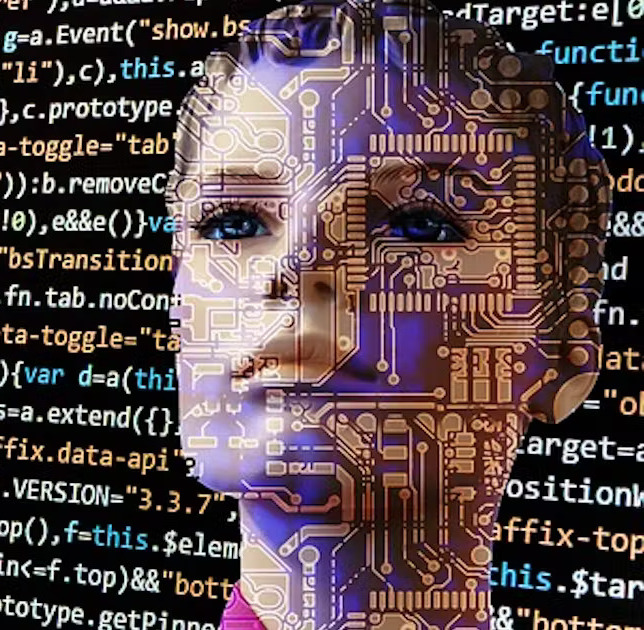
\includegraphics[width=.9\linewidth]{images/ib.jpg}
\end{center}
\end{threec}
\end{frame}

\begin{frame}[label={sec:org0122229}]{Tipos de IAs - P1}
\begin{block}{Tipo-1: Basado en su capacidad \footnote{\autocite{Jones_2009}}}
\begin{block}{Narrow AI}
Inteligencias artificiales de dominio limitado
\end{block}

\begin{block}{General AI}
Asemeja la forma de pensar y razonar del humano. No existe
\end{block}

\begin{block}{Strong AI}
Supera la inteligencia del humano. No existe
\end{block}
\end{block}
\end{frame}

\begin{frame}[label={sec:orgcf4bb3e}]{Tipos de IAs - P2}
\begin{block}{Tipo-2: Basado en su funcionalidad \footnote{\autocite{Jones_2009}}}
\begin{block}{Reactive machines}
Sin memoria, reaccionan a entradas y producen salidas
\end{block}

\begin{block}{Limited memory}
Tienen memoria limitada y toman decisiones basadas en acciones previas
\end{block}

\begin{block}{Theory of mind}
Intentan comprender la mente humana para emular el pensamiento humano
\end{block}
\end{block}
\end{frame}

\begin{frame}[label={sec:orgc9e4388}]{Ramas de la IA}
\begin{figure}[htbp]
\centering
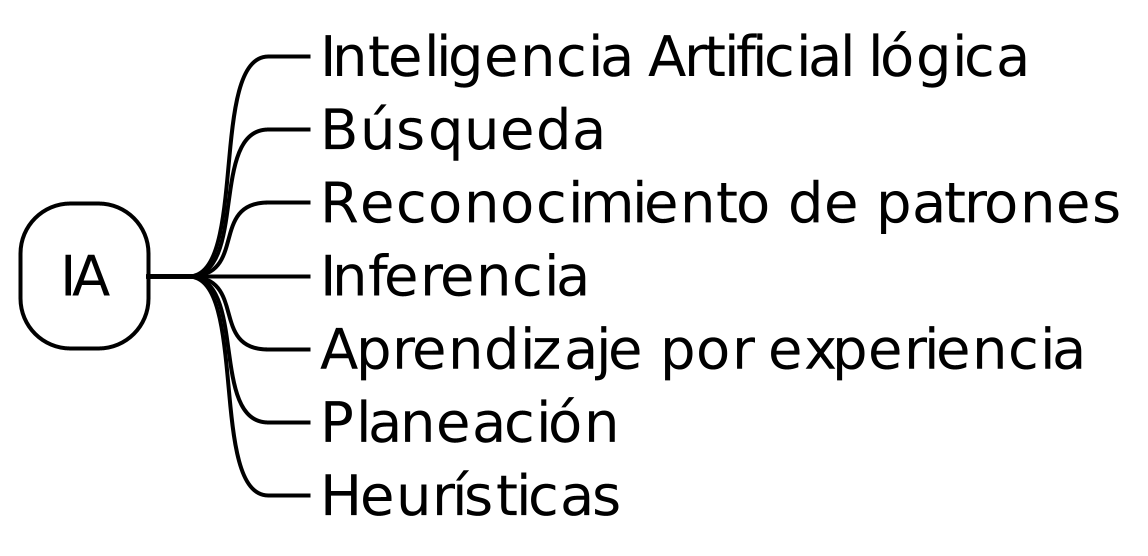
\includegraphics[height=100px]{./images/mp.png}
\caption{Algunas áreas de las ramas de la IA}
\end{figure}
\end{frame}

\begin{frame}[label={sec:org2cc85b8}]{Aplicaciones de IA actuales}
\begin{block}{Algunos usos actuales\footnote{\autocite{Biswal_2023}}}
\begin{twoc}
\begin{itemize}
\item Navegacion GPS
\item Creación de Contenido Inteligente
\item Asistentes de Voz
\item Vehículos Autónomos
\item Reconocimiento Facial
\item Sistema de Recomendación
\end{itemize}
\end{twoc}
\begin{threec}
\begin{figure}[htbp]
\centering
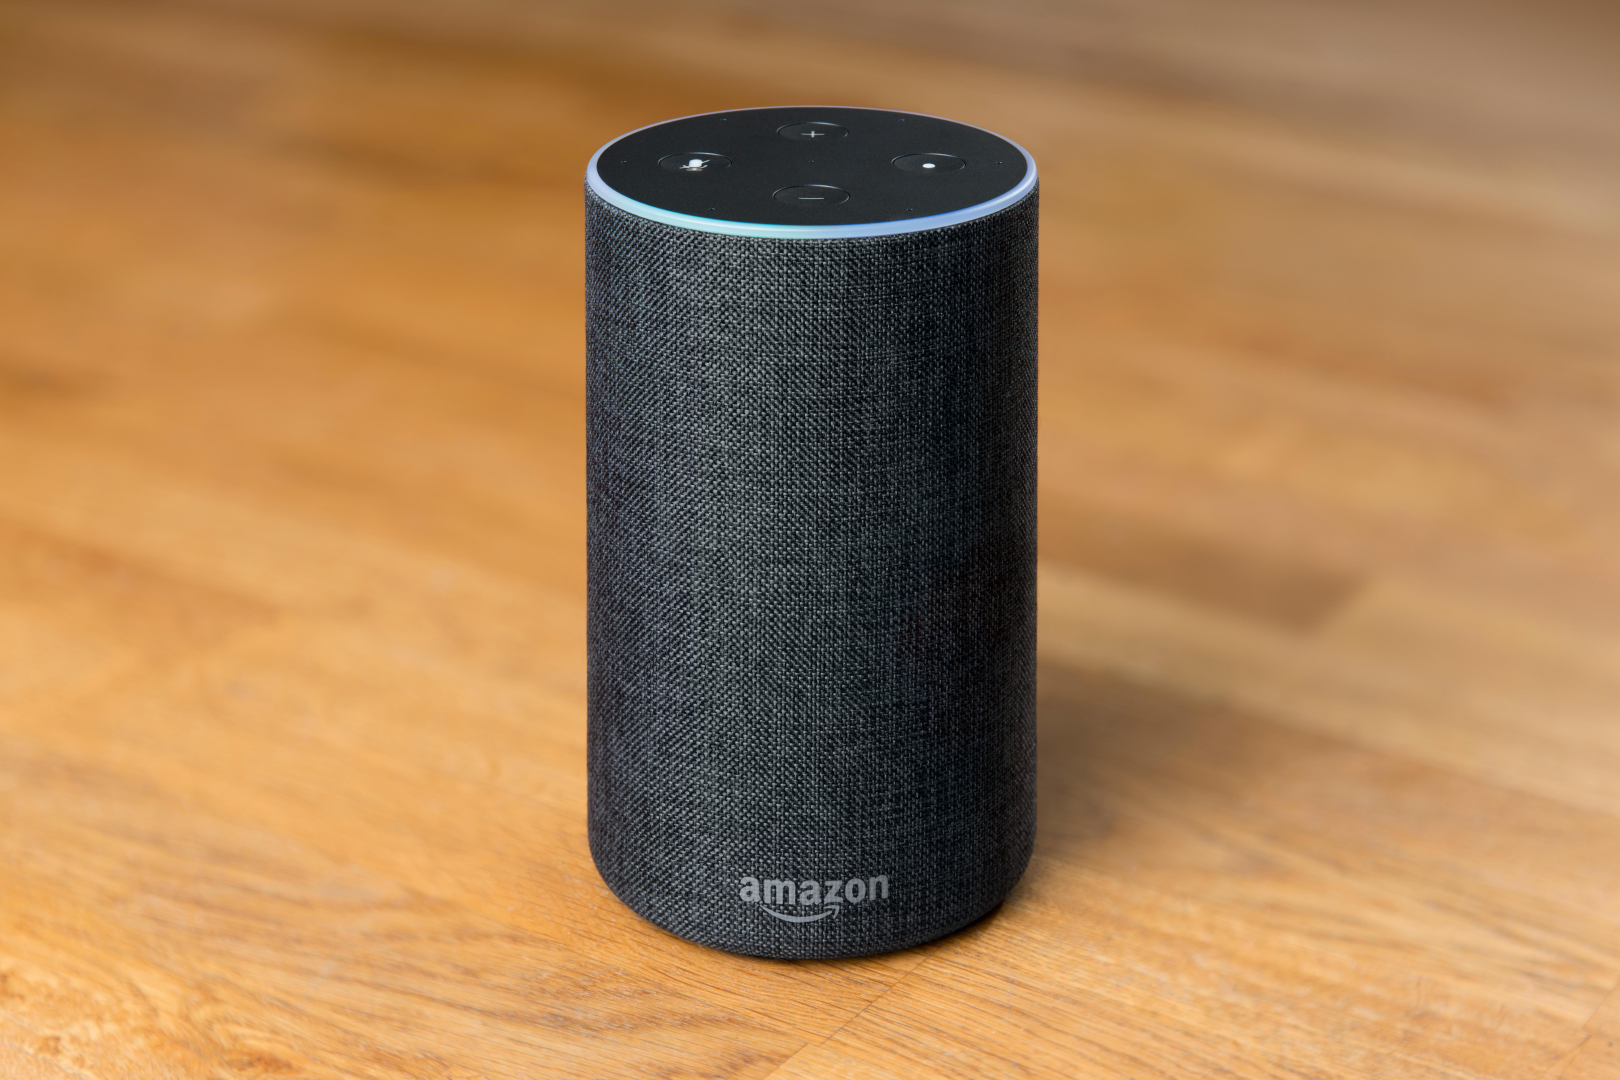
\includegraphics[width=.9\linewidth]{images/alexa.png}
\caption{Amazon Alexa}
\end{figure}
\end{threec}
\end{block}
\end{frame}

\begin{frame}[label={sec:org6eb8e1d}]{Relación de aplicación con el proyecto}
\begin{threec}
\alert{Detalles} \\
El proyecto que estamos desarrollando es un software para gestionar un hospital
diagnosticar al paciente es de las tareas mas criticas que ejerce un médico
un mal diagnostico puede comprometer por completo la salud del paseante

\begin{center}
\begin{tabular}{l}
\\
\end{tabular}

\end{center}

\alert{Propuesta} \\
Un sistema experto podría ayudar al diagnostico de paciente, es importante 
recalcar que no se pretende reemplazar al doctor si no apoyar utilizando
los datos de diagnósticos previos para poder explorar la mayor cantidad posible
de enfermedades.
\end{threec}
\begin{twoc}
\begin{center}
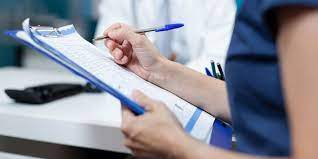
\includegraphics[width=.9\linewidth]{images/diag.jpeg}
\end{center}
\end{twoc}
\end{frame}


\begin{frame}[label={sec:orgd735547}]{Referencias}
\printbibliography
\end{frame}
\end{document}
